\documentclass{beamer}
\usetheme{Boadilla}

\usepackage{amsmath}
\usepackage{amsfonts}
\usepackage{hyperref}

\usepackage[style=verbose,backend=biber]{biblatex}
\addbibresource{ref.bib}

\title{SSM}
\author{Skorik Sergey}
\institute{MIPT, 2023}


\begin{document}

% \begin{frame}
%     \titlepage
% \end{frame}

% \begin{frame}
%     \tableofcontents
% \end{frame}

\section{Project 1}

\begin{frame}{Project 1}
    \begin{block}{Plan}
        \begin{itemize}
            \item \textbf{Title:} Spatial time series reconstruction using structured state spaces (\href{https://arxiv.org/abs/2111.00396}{S4})
            \item \textbf{Problem:} Consider spatial time-series signal $\mathbf{X}\in\mathbb{R}^{E\times N}$. Find Optimal state space $\mathbf{x}$ that has best reconstructs $\mathbf{X}'$ (in terms of reconstruction loss).
            \item \textbf{Data:} Any of the available EEG datasets, e.g. \href{https://neurotechx.github.io/moabb/generated/moabb.datasets.PhysionetMI.html#moabb.datasets.PhysionetMI}{PhysionetMI}
            \item \textbf{Base solution:} take existing baselines for reconstruction
            \item \textbf{Proposed solution:} Use S4 layer as the building block of the seq2seq models.
            \item \textbf{Novelty:} Novelty to be clarified, but S4 layers have recently appeared and there are few studies that have examined them for EEG
        \end{itemize}
    \end{block}
\end{frame}

\begin{frame}{S4}
    \begin{figure}
        \centering
        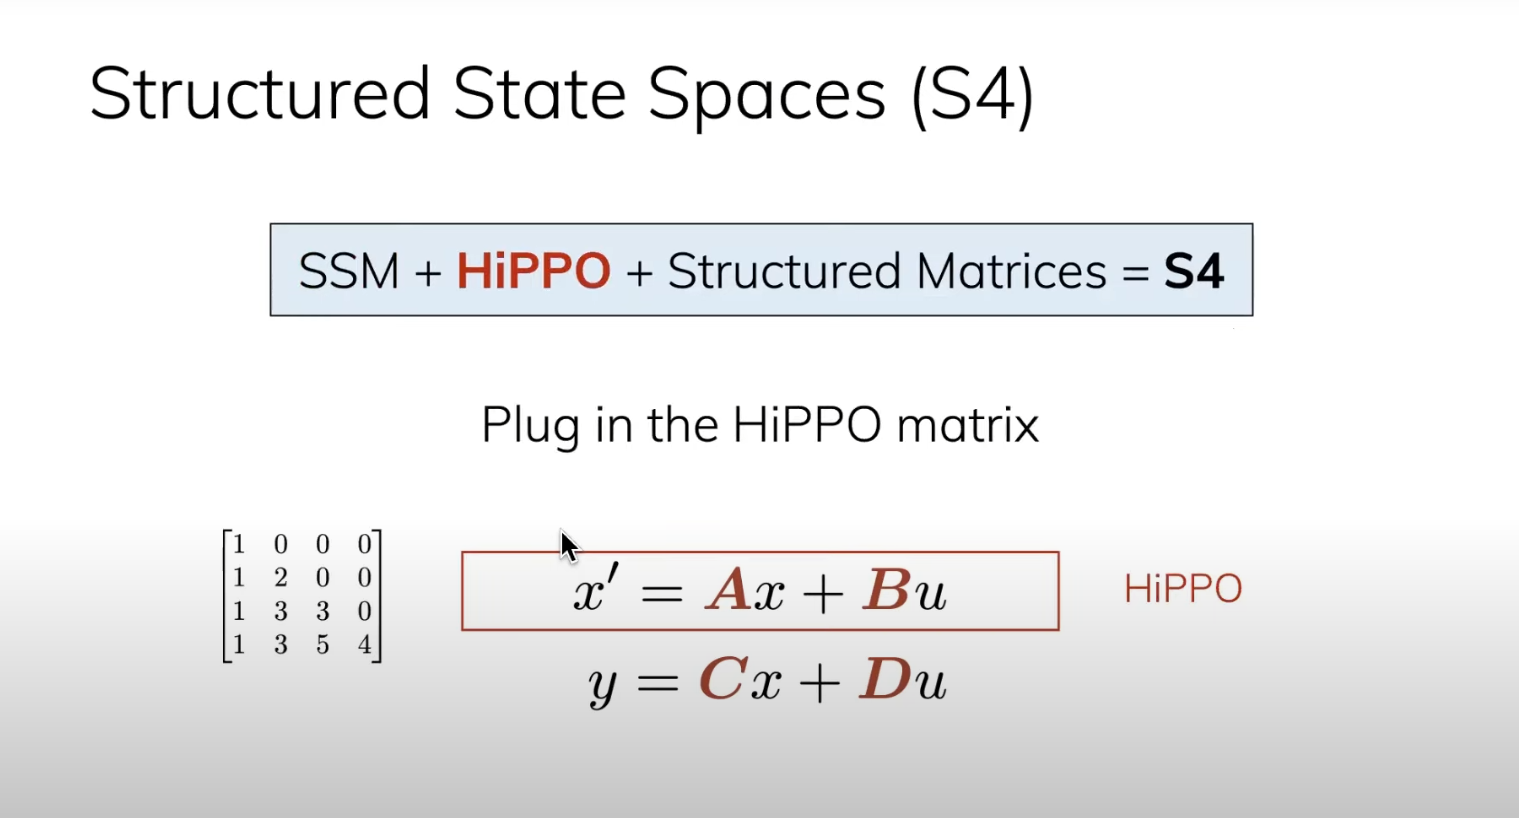
\includegraphics[width=\textwidth]{S4.png}
    \end{figure}
\end{frame}

\begin{frame}{S4}
    \begin{figure}
        \centering
        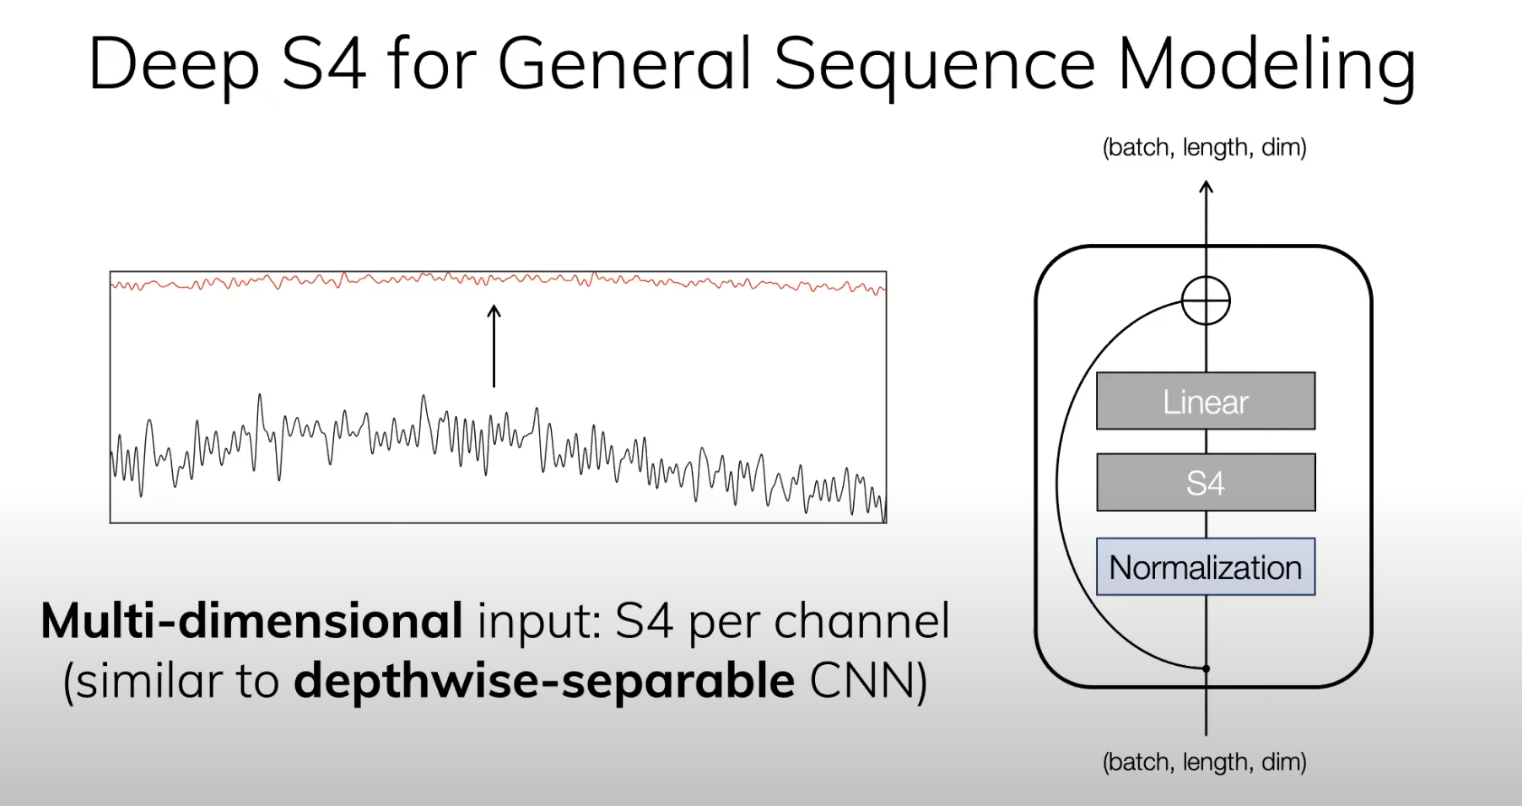
\includegraphics[width=\textwidth]{S4_deep.png}
    \end{figure}
\end{frame}
\end{document}
